\chapter{Resultados}

En este capitulo se exponen los resultados

<<<<<<< HEAD
=======
<<<<<<< HEAD
>>>>>>> master
\section{Alumnos}
%---------------------------------------------------------
\section{Docente}
%---------------------------------------------------------
\section{Personal de seguridad}

Se analizaron 15 respuestas del personal de seguridad sobre el uso de la aplicación móvil para la verificación de credenciales estudiantiles mediante códigos QR. Los resultados reflejan una percepción mayormente positiva, aunque se identificaron áreas clave de mejora, particularmente en la visualización de datos y la consistencia del escaneo.

A continuación se detalla el análisis completo:

\subsection{Facilidad de uso del escaneo del código QR}

\begin{itemize}
	\item \textbf{Facilidad de escaneo:} 
	El 60\% de los usuarios calificó la experiencia como \textbf{Muy fácil} y el 33.3\% como \textbf{Fácil} (ver gráfica~\ref{fig:facilidad-escaneo}). 
	Solo un 6.7\% \textbf{Muy difícil} reportó problemas técnicos, donde la aplicación tardó 10 segundos en detectar el QR (de acuerdo con el comentario del usuario, por baja iluminación en su entorno).
	
	\begin{figure}[H]
		\centering
		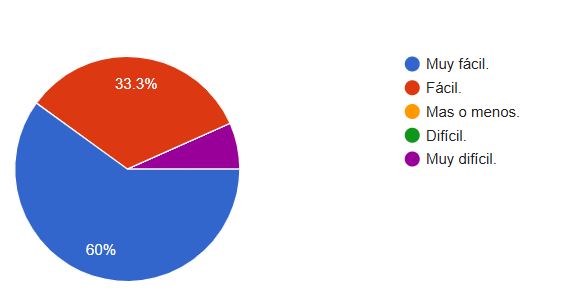
\includegraphics[width=0.7\textwidth]{images/grafico_escaneo.png}
		\caption{Distribución de respuestas sobre la facilidad de escaneo del código QR.}
		\label{fig:facilidad-escaneo}
	\end{figure}
	
	\item \textbf{Tiempo de lectura del QR:}  
	El 46.7\% de los usuarios (7/15) reportó un tiempo de escaneo de 5 segundos, mientras que el 33.3\% (5/15) observó 2 segundos y el 20\% (3/15) tardó 10 segundos (ver gráfica~\ref{fig:tiempo-escaneo}).  
	Aunque el 80\% de los casos se resolvió en 5 segundos, los tiempos mayores (10s) sugieren la necesidad de optimizar el procesamiento en dispositivos antiguos o con baja iluminación, así como la conexión a internet.
	
	\begin{figure}[H]
		\centering
		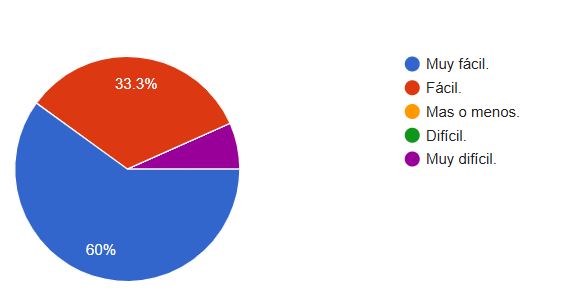
\includegraphics[width=0.7\textwidth]{images/grafico_escaneo.png}
		\caption{Distribución de respuestas sobre el tiempo de escaneo del código QR.}
		\label{fig:tiempo-escaneo}
	\end{figure}
	
	\item \textbf{Precisión del escaneo QR:} 
	La aplicación funciona correctamente en la mayoría de los casos, con 13 de 15 usuarios (87\%) calificando su precisión como buena o excelente (4-5 puntos de 5). 
	Solo 2 usuarios reportaron dificultades ocasionales, como que \textbf{la cámara no reconocía el código inmediatamente}. Esto indica que, aunque el sistema es confiable, existen oportunidades para hacer el proceso aún más consistente para todos los usuarios.
\end{itemize}

\subsection{Visualización de la información}
\textbf{Legibilidad de la información:}  
La mayoría de los usuarios calificaron positivamente la claridad de la información (4-5 puntos en una escala de 5), lo que demuestra que el diseño general es efectivo.  
Sin embargo, varios usuarios reportaron problemas específicos con la visualización completa de los datos, comentando que: \textbf{los datos de la credencial del alumno no se muestran completos} y \textbf{la información aparece cortada}. Estos comentarios señalan la necesidad de ajustar el formato de visualización de la credencial del alumno para garantizar que toda la información sea visible.

\subsection{Experiencia de usuario}

\begin{itemize}
	\item \textbf{Navegación:}  
	El 100\% de los usuarios (15 de 15) calificaron con 4 o 5 puntos (en una escala de 5) la facilidad de navegación en la aplicación. De ellos, 8 usuarios (53.3\%) asignaron una calificación de 4 y 7 usuarios (46.7\%) otorgaron una calificación de 5, lo que refleja una percepción positiva generalizada sobre la usabilidad del sistema (ver gráfica~\ref{fig:navegacion}).
	
	\begin{figure}[H]
		\centering
		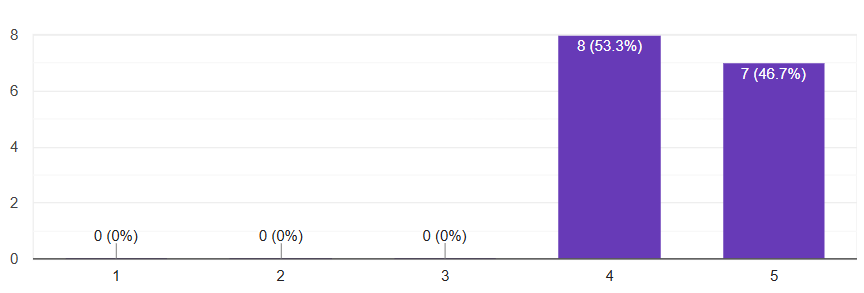
\includegraphics[width=0.7\textwidth]{images/navegacion.png}
		\caption{Evaluación de la experiencia de navegación en la aplicación.}
		\label{fig:navegacion}
	\end{figure}
	
	\item \textbf{Colores:}  
	La evaluación del esquema de colores fue mayormente positiva, con puntuaciones entre 4 y 5. El 53.3\% de los usuarios lo calificó con la máxima puntuación (5), mientras que el 46.7\% lo valoró con un 4 (ver gráfica~\ref{fig:colores}).
	
	\begin{figure}[H]
		\centering
		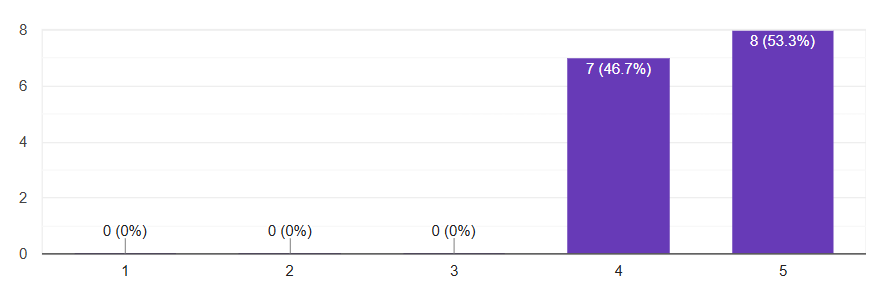
\includegraphics[width=0.7\textwidth]{images/colores.png}
		\caption{Evaluación del esquema de colores por los usuarios.}
		\label{fig:colores}
	\end{figure}
	
<<<<<<< HEAD
	
=======


>>>>>>> master
	\item \textbf{Comodidad para tomar asistencia:}  
	La mayoría de los usuarios calificó la experiencia con una puntuación de 4 a 5 en una escala de 5, lo que indica una alta aceptación y satisfacción con el proceso de toma de asistencia mediante la aplicación. Esto sugiere que el sistema es intuitivo y facilita la labor del personal de seguridad al momento de registrar la asistencia de los alumnos.
\end{itemize}

\subsection{Efectividad contra suplantación de identidad}

La mayoría de los usuarios (93.4\%) consideró que la aplicación sería muy efectiva para evitar la suplantación de identidad durante los ETS, otorgando calificaciones altas (8-10 puntos en una escala de 10). Los resultados detallados fueron (ver gráfica~\ref{fig:efectividad}):

\begin{itemize}
	\item \textbf{(68.7\%):} Máxima efectividad, destacando la utilidad del sistema QR como un método para evitar la suplantación de identidad.
	\item \textbf{(26.7\%):} Efectividad moderada, con sugerencias para implementar verificaciones adicionales.
	\item \textbf{(6.7\%):} Baja percepción de efectividad.
\end{itemize}

\begin{figure}[H]
	\centering
	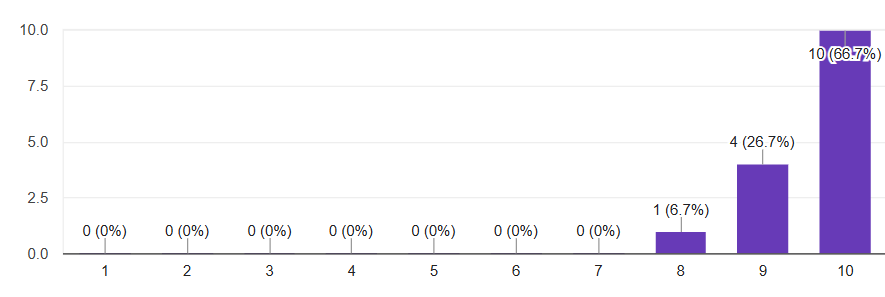
\includegraphics[width=0.7\textwidth]{images/efectividad.png}
	\caption{Evaluación de usuarios sobre la efectividad del sistema QR contra suplantación de identidad.}
	\label{fig:efectividad}
\end{figure}
<<<<<<< HEAD
=======
=======

\section{Alumnos}
De la sección de los alumnos, se analizaron 41 resultados sobre el uso de la aplicación móvil, tanto para probar el reconocimiento, como para ver el listado de los ETS existentes. 
Los resultados, en su mayor parte, son comentarios positivos, sin embargo, a lo largo del desarrollo de las pruebas salieron a relucir varios puntos de mejora sobre la aplicación, en su mayor parte de visualización
.

A continuación se detalla el análisis completo:
\subsection{Facilidad de uso del escaneo del código QR}
\begin{itemize}
	\item \textbf{Facilidad de escaneo:} 
	El 60\% de los usuarios calificó la experiencia como \textbf{Muy fácil} y el 33.3\% como \textbf{Fácil} (gráfica~\ref{fig:facilidad-escaneo}). 
	Solo un 6.7\% \textbf{Muy difícil} reportó problemas técnicos, donde la aplicación tardó 10 segundos en detectar el QR (de acuerdo con el comentario del usuario, por baja iluminación en su entorno).
	
	\begin{figure}
		\centering
		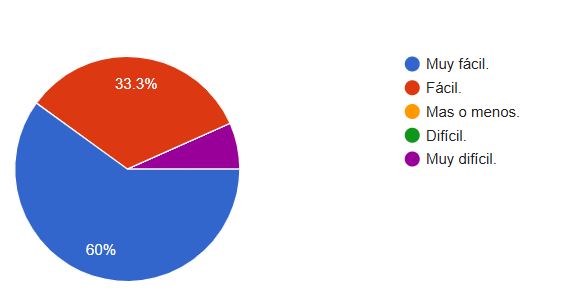
\includegraphics[width=0.7\textwidth]{images/grafico_escaneo.png}
		\caption{Distribución de respuestas sobre la facilidad de escaneo del código QR.}
		\label{fig:facilidad-escaneo}
	\end{figure}
	
	\item \textbf{Tiempo de lectura del QR:}  
	El 46.7\% de los usuarios (7/15) reportó un tiempo de escaneo de 5 segundos, mientras que el 33.3\% (5/15) observó 2 segundos y el 20\% (3/15) tardó 10 segundos (gráfica~\ref{fig:tiempo-escaneo}).  
	Aunque el 80\% de los casos se resolvió en 5 segundos, los tiempos mayores (10s) sugieren la necesidad de optimizar el procesamiento en dispositivos antiguos o con baja iluminación, así como la conexión a internet.
	
	\begin{figure}
		\centering
		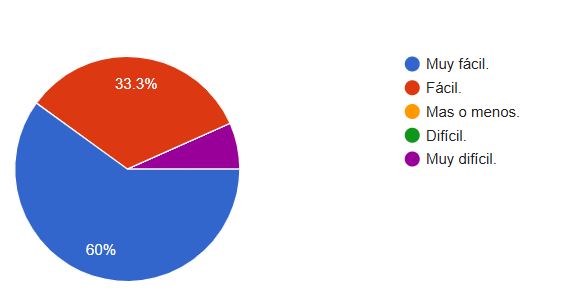
\includegraphics[width=0.7\textwidth]{images/grafico_escaneo.png}
		\caption{Distribución de respuestas sobre el tiempo de escaneo del código QR.}
		\label{fig:tiempo-escaneo}
	\end{figure}
	
	\item \textbf{Precisión del escaneo QR:} 
	La aplicación funciona correctamente en la mayoría de los casos, con 13 de 15 usuarios (87\%) calificando su precisión como buena o excelente (4-5 puntos de 5). 
	
	Solo 2 usuarios reportaron dificultades ocasionales, como que \textbf{la cámara no reconocía el código inmediatamente}. Esto indica que, aunque el sistema es confiable, existen oportunidades para hacer el proceso aún más consistente para todos los usuarios.
\end{itemize}

\subsection{Visualización de la información}
\textbf{Legibilidad de la información:} 
La mayoría de los usuarios calificaron positivamente la claridad de la información (4-5 puntos en una escala de 5), lo que demuestra que el diseño general es efectivo.
Sin embargo, varios usuarios reportaron problemas específicos con la visualización completa de los datos, comentando que: \textbf{los datos de la credencial del alumno no se muestran completos} y \textbf{la información aparece cortada}. Estos comentarios señalan la necesidad de ajustar el formato de visualización de la credencial del alumno para garantizar que toda la información sea visible.
%---------------------------------------------------------
\section{Docentes}

En esta sección, se presenta el análisis exhaustivo de los resultados obtenidos de las 15 encuestas realizadas a docentes. Estas encuestas tuvieron como propósito principal evaluar tanto el funcionamiento como la experiencia de uso de la aplicación móvil en funcionalidades clave. La recolección de esta retroalimentación es crucial para comprender a fondo la percepción de los usuarios sobre aspectos críticos del sistema y su desempeño en un entorno real. 

Las preguntas de las encuestas se diseñaron para enfocarse en varios puntos específicos: la efectividad del reconocimiento facial, la facilidad y precisión para consultar el listado de ETS y la eficiencia en la comparación de credenciales mediante código QR. 

Los resultados preliminares de estas encuestas, en sintonía con la retroalimentación de otros grupos de usuarios, arrojan una mayoría de comentarios positivos respecto a la operatividad general de las funcionalidades. Sin embargo, el proceso de encuestado también permitió identificar puntos específicos de mejora y áreas de oportunidad significativas. Estas incluyen tanto aspectos relacionados con la usabilidad y la experiencia del usuario, como la detección de errores de funcionalidad específicos que se detallan en la sección de pruebas.

A continuación, se presenta el análisis completo de las encuestas aplicadas a los docentes, desglosando los hallazgos y las implicaciones para futuras mejoras del sistema. 

%---------------------------------------------------------

\section{Personal de seguridad}

Se analizaron 15 respuestas del personal de seguridad sobre el uso de la aplicación móvil para la verificación de credenciales estudiantiles mediante códigos QR. Los resultados reflejan una percepción mayormente positiva, aunque se identificaron áreas clave de mejora, particularmente en la visualización de datos y la consistencia del escaneo.

A continuación se detalla el análisis completo:

\subsection{Facilidad de uso del escaneo del código QR}

\begin{itemize}
	\item \textbf{Facilidad de escaneo:} 
	El 60\% de los usuarios calificó la experiencia como \textbf{Muy fácil} y el 33.3\% como \textbf{Fácil} (ver gráfica~\ref{fig:facilidad-escaneo}). 
	Solo un 6.7\% \textbf{Muy difícil} reportó problemas técnicos, donde la aplicación tardó 10 segundos en detectar el QR (de acuerdo con el comentario del usuario, por baja iluminación en su entorno).
	
	\begin{figure}[H]
		\centering
		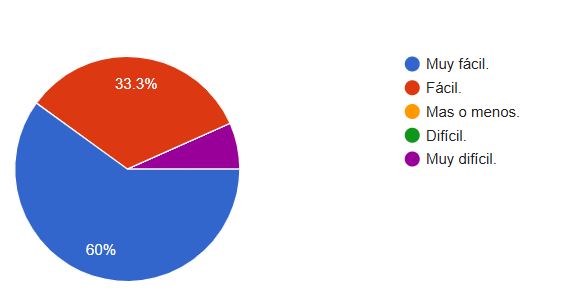
\includegraphics[width=0.7\textwidth]{images/grafico_escaneo.png}
		\caption{Distribución de respuestas sobre la facilidad de escaneo del código QR.}
		\label{fig:facilidad-escaneo}
	\end{figure}
	
	\item \textbf{Tiempo de lectura del QR:}  
	El 46.7\% de los usuarios (7/15) reportó un tiempo de escaneo de 5 segundos, mientras que el 33.3\% (5/15) observó 2 segundos y el 20\% (3/15) tardó 10 segundos (ver gráfica~\ref{fig:tiempo-escaneo}).  
	Aunque el 80\% de los casos se resolvió en 5 segundos, los tiempos mayores (10s) sugieren la necesidad de optimizar el procesamiento en dispositivos antiguos o con baja iluminación, así como la conexión a internet.
	
	\begin{figure}[H]
		\centering
		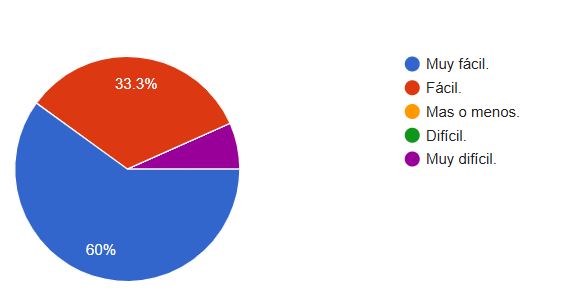
\includegraphics[width=0.7\textwidth]{images/grafico_escaneo.png}
		\caption{Distribución de respuestas sobre el tiempo de escaneo del código QR.}
		\label{fig:tiempo-escaneo}
	\end{figure}
	
	\item \textbf{Precisión del escaneo QR:} 
	La aplicación funciona correctamente en la mayoría de los casos, con 13 de 15 usuarios (87\%) calificando su precisión como buena o excelente (4-5 puntos de 5). 
	Solo 2 usuarios reportaron dificultades ocasionales, como que \textbf{la cámara no reconocía el código inmediatamente}. Esto indica que, aunque el sistema es confiable, existen oportunidades para hacer el proceso aún más consistente para todos los usuarios.
\end{itemize}

\subsection{Visualización de la información}
\textbf{Legibilidad de la información:}  
La mayoría de los usuarios calificaron positivamente la claridad de la información (4-5 puntos en una escala de 5), lo que demuestra que el diseño general es efectivo.  
Sin embargo, varios usuarios reportaron problemas específicos con la visualización completa de los datos, comentando que: \textbf{los datos de la credencial del alumno no se muestran completos} y \textbf{la información aparece cortada}. Estos comentarios señalan la necesidad de ajustar el formato de visualización de la credencial del alumno para garantizar que toda la información sea visible.

\subsection{Experiencia de usuario}

\begin{itemize}
	\item \textbf{Navegación:}  
	El 100\% de los usuarios (15 de 15) calificaron con 4 o 5 puntos (en una escala de 5) la facilidad de navegación en la aplicación. De ellos, 8 usuarios (53.3\%) asignaron una calificación de 4 y 7 usuarios (46.7\%) otorgaron una calificación de 5, lo que refleja una percepción positiva generalizada sobre la usabilidad del sistema (ver gráfica~\ref{fig:navegacion}).
	
	\begin{figure}[H]
		\centering
		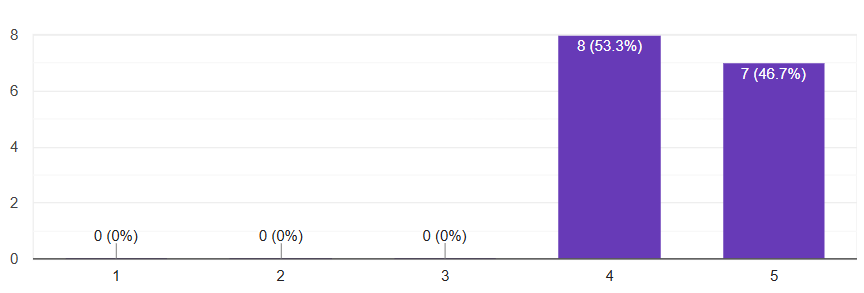
\includegraphics[width=0.7\textwidth]{images/navegacion.png}
		\caption{Evaluación de la experiencia de navegación en la aplicación.}
		\label{fig:navegacion}
	\end{figure}
	
	\item \textbf{Colores:}  
	La evaluación del esquema de colores fue mayormente positiva, con puntuaciones entre 4 y 5. El 53.3\% de los usuarios lo calificó con la máxima puntuación (5), mientras que el 46.7\% lo valoró con un 4 (ver gráfica~\ref{fig:colores}).
	
	\begin{figure}[H]
		\centering
		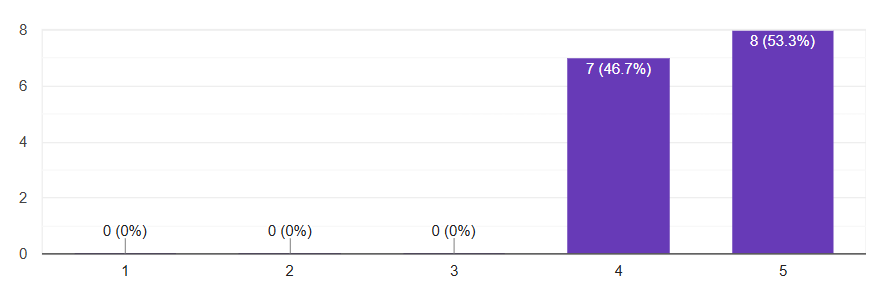
\includegraphics[width=0.7\textwidth]{images/colores.png}
		\caption{Evaluación del esquema de colores por los usuarios.}
		\label{fig:colores}
	\end{figure}
	
	\item \textbf{Comodidad para tomar asistencia:}  
	La mayoría de los usuarios calificó la experiencia con una puntuación de 4 a 5 en una escala de 5, lo que indica una alta aceptación y satisfacción con el proceso de toma de asistencia mediante la aplicación. Esto sugiere que el sistema es intuitivo y facilita la labor del personal de seguridad al momento de registrar la asistencia de los alumnos.
\end{itemize}

\subsection{Efectividad contra suplantación de identidad}

La mayoría de los usuarios (93.4\%) consideró que la aplicación sería muy efectiva para evitar la suplantación de identidad durante los ETS, otorgando calificaciones altas (8-10 puntos en una escala de 10). Los resultados detallados fueron (ver gráfica~\ref{fig:efectividad}):

\begin{itemize}
	\item \textbf{(68.7\%):} Máxima efectividad, destacando la utilidad del sistema QR como un método para evitar la suplantación de identidad.
	\item \textbf{(26.7\%):} Efectividad moderada, con sugerencias para implementar verificaciones adicionales.
	\item \textbf{(6.7\%):} Baja percepción de efectividad.
\end{itemize}

\begin{figure}[H]
	\centering
	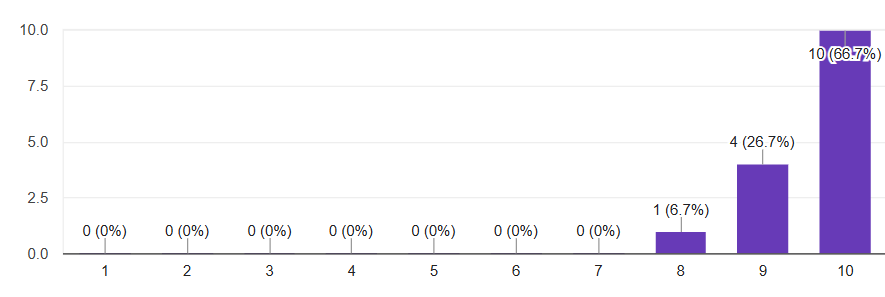
\includegraphics[width=0.7\textwidth]{images/efectividad.png}
	\caption{Evaluación de usuarios sobre la efectividad del sistema QR contra suplantación de identidad.}
	\label{fig:efectividad}
\end{figure}

>>>>>>> a80c0535ff7ff92f5be9b35087c8d40e853f42a8
>>>>>>> master
